\subsection*{Partie I}
\begin{enumerate} \item \begin{enumerate}
 \item Si $g$ est strictement croissante, $E=]a,b[$.
 \item Si $a=-1$, $b=1$ et $g(t) = 1-t^2$ alors $E=]-1,0[ $.
 \item Si $a=0$, $b=2\pi$ et $g(t) = sin(t)$, alors $E=] 0,\frac{\pi }{2}[ \, \cup \, ] \pi,2\pi [$.
 \item On calcule la d{\'e}riv{\'e}e : $g^{\prime}(x)=2x(-2x^{2}+1)$. On en déduit les variations et l'allure du graphe (figure \ref{Clebesg_1}) de la fonction définie par $g(t)=-t^{4}+t^{2}$. 
\begin{figure}[ht]
\centering
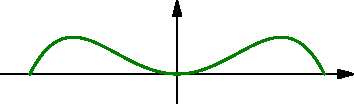
\includegraphics{Clebesg_1.pdf}
\caption{Question I.1.d.}
\label{Clebesg_1}
\end{figure}
On en tire
\begin{displaymath}
 E = \left]-1,-\frac{1}{\sqrt{2}}\right[  \cup \left] -\frac{1}{\sqrt{2}},\frac{1}{\sqrt{2}} \right[ 
\end{displaymath}
\end{enumerate}

\item En choisissant les points o{\`u} la d{\'e}riv{\'e}e change de signe on choisit les extrema locaux. Prenons par exemple la fonction dont la d{\'e}riv{\'e}e est 
\begin{displaymath}
 t\rightarrow (t-0.7)(t-1.5)
\end{displaymath}
dans l'intervalle $[0,2]$ (graphe en figure \ref{Clebesg_2}).
\begin{figure}[ht]
\centering
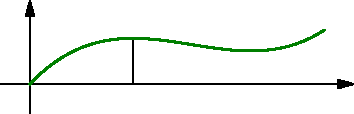
\includegraphics{Clebesg_2.pdf}
\caption{question I.2 $E$ contient un maximum local.}
\label{Clebesg_2}
\end{figure}

Pour une telle fonction, $E = \left] 0,2 \right[$ et contient le maximum local en $0.7$ car ce n'est pas le maximum global de la fonction.

\item Une fonction strictement d{\'e}croissante dans $]a,b]$ ne l'est pas forc{\'e}ment  dans $[a,b] $ car la valeur de $f(a) $ peut {\^e}tre quelconque.
 Si on suppose en plus la continuit{\'e} en $a$, la valeur de $f(a)$ est alors la limite {\`a} droite en $a$ soit $\sup_{] a,b] }f$. La fonction $f$ est alors d{\'e}croissante dans $[ a,b] $.\newline
Cette d{\'e}croissance est stricte car, si $f(a)=f(c)$ pour un $c$ de $] a,b]$, la fonction $f$ serait alors constante sur $]a,c]$.
\item \begin{enumerate}
 \item L'ensemble $E$ est vide si et seulement si
\begin{displaymath}
 \forall x \in ]a,b[ , \forall y \in ]x,b] : g(x)\leq g(y)
\end{displaymath}
Ceci traduit exactement la d{\'e}croissance de $g$ dans $] a,b] $. Comme $g$ est continue dans $[ a,b] $, c'est {\'e}quivalent {\`a} la d{\'e}croissance de $g$ dans $[a,b]$.
\item  La fonction continue $g$ atteint sa borne sup{\'e}rieure $M$ sur le segment $[a,b]$ en un point $x_{\max }$. Il est clair que $x_{\max}\notin E$ donc $x_{\max }\in \left\lbrace a,b\right\rbrace $ et $M\in \left\lbrace g(a),g(b)\right\rbrace$.\newline
Les deux cas possibles sont $g(a)<g(b)=M$ et $g(a)=g(b)=M$.\newline
Ils sont illustr{\'e}s par les graphes des fonctions $1+(t-0.4)^2$ (figure \ref{Clebesg_3}) et $1-(t-0.5)^2$ (figure \ref{Clebesg_4} ) sur $[0,1]$.
\begin{figure}[ht]
\centering
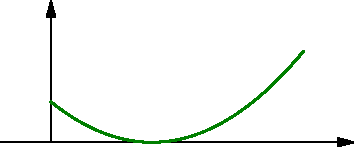
\includegraphics{Clebesg_3.pdf} 
\caption{Cas 2. $g(a)<M=g(b)$}
\label{Clebesg_3}
\end{figure}
\begin{figure}[ht]
\centering
 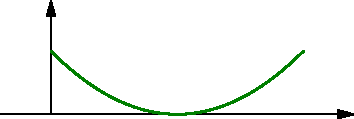
\includegraphics{Clebesg_4.pdf}
\caption{Cas 1. $M=g(a)=g(b)$}
\label{Clebesg_4}
\end{figure}

 La r{\'e}ciproque n'est pas vraie. Une relation $M=g(a)$ ou $g(b)$ n'emp{\^e}che pas que le maximum puisse {\^e}tre atteint en un autre point {\`a} l'int{\'e}rieur du segment. Dans ce cas $E$ ne sera pas $]a,b[ $. On peut choisir par exemple la fonction $\cos$ sur $[0,4\pi]$.
\begin{figure}[ht]
\centering
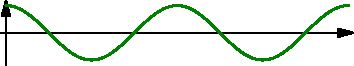
\includegraphics[width=7cm]{Clebesg_5.pdf}
\caption{Cas où $g(a)= M = g(B)$ et  $E$ n'est pas $]a,b[$.}
\end{figure}
\end{enumerate}
\end{enumerate}

\subsection*{Partie II}
\begin{enumerate}
 \item Quand $x$ augmente, l'intervalle $[ x,b] $ se r{\'e}duit. La fonction $\Psi $ est donc d{\'e}croissante.\newline
 Pour {\'e}tudier la continuit{\'e} de $\Psi$, deux méthodes sont possibles.\newline
La première consiste en une étude locale autour d'un point $x$ de $[a,b[ $.\newline
Remarquons d'abord que la fonction continue $g$ atteint sa borne sup{\'e}rieure sur $[x,b] $. Il existe donc $m\in [x,b]$ tel que $\Psi (x)=g(m)$. Distinguons deux cas.
\begin{description}
 \item[Cas 1.] $\Psi (x)=g(m)>g(x)$.\newline
Alors $m\in ] x,b] $ et par continuité en $x$,  il existe $\alpha >0$ tel que
\begin{displaymath}
 \forall t \in [x-\alpha,x]  : g(t)<g(m)
\end{displaymath}
On en d{\'e}duit que $\Psi(y)=\Psi(x)$ lorsque $y\in [x-\alpha ,m]$. Ainsi, la fonction $\Psi $ est non seulement continue mais \emph{constante} au voisinage de $x$.
\item[Cas 2.] $\Psi (x)=g(m)=g(x)$.\newline
Par continuit{\'e} de $g$ en $x$, pour tout $\varepsilon >0$, il existe un $\alpha >0$ tel que 
\begin{displaymath}
 \forall t\in [x-\alpha ,x+\alpha]  :  \Psi(x)-\varepsilon \leq g(t)\leq \Psi (x)+\varepsilon 
\end{displaymath}
On va alors chercher à encadrer $\Psi(y)$ pour $y\in [x-\alpha ,x+\alpha]$.\newline
Utilisons d'abord d{\'e}croissance de $\Psi$ :
\begin{displaymath}
\forall y\in [x-\alpha ,x+\alpha] : \Psi(x+\alpha )\leq \Psi(y)\leq \Psi (x-\alpha)
\end{displaymath}
D'un côté :
\begin{align*}
\forall t\in [ x-\alpha ,x] &:& g(t)\leq \Psi (x)+\varepsilon \\
\forall t\in [ x,b] &:& g(t)\leq \Psi (x)
\end{align*}
ce qui entra\^{\i }ne $\Psi (x-\alpha )\leq \Psi (x)+\varepsilon$.\newline
De l'autre 
\begin{displaymath}
 \Psi(x)-\varepsilon \leq g(x+\alpha)\leq \Psi(x+\alpha)
\end{displaymath}
ce qui entra\^{\i }ne $\Psi (x)-\varepsilon\leq \Psi(x+\alpha)$.\newline
Finalement on a donc 
\begin{displaymath}
 \forall y\in [x-\alpha ,x+\alpha] : \Psi (x)-\varepsilon\leq \Psi(x+\alpha) \leq \Psi(y)\leq \Psi (x-\alpha )\leq \Psi (x)+\varepsilon
\end{displaymath}
ce qui assure la continuité de $\Psi$ en $x$.
\end{description}
Une deuxième méthode possible consiste à utiliser un résultat de cours sur les fonctions monotones. Si $f$ est une fonction monotone définie sur un intervalle $I$ et si $f(I)$ est un intervalle, alors $f$ est continue dans $I$. Ce résultat repose sur l'étude des limites des fonctions monotones. Il sert en particulier à prouver la continuité de la bijection réciproque d'une fonction bijective, monotone et continue sur un intervalle.\newline
Il faudrait alors montrer que l'image par $\psi$ de l'intervalle $[a,b]$ est un intervalle.\newline
La fonction $g$ est continue sur un segment donc bornée. Notons
\begin{displaymath}
 M=g(x_m)=\max_{[a,b]}g
\end{displaymath}
Il est clair que $\Psi$ est à valeurs dans $[M,g(b)]$. On doit montrer que, pour tout $y$ dans $[M,g(b)]$, il existe un $x\in [a,b]$ tel que $\Psi(x)=y$. Cette méthode ne sera pas développée davantage.

\item \begin{enumerate}
 \item Un {\'e}l{\'e}ment $x$ de $] a,b[ $ est dans $E$ si et seulement si $g(x)<\Psi (x)$.
 
 \item Si $x\in E$, on sait que 
\begin{displaymath}
\dfrac{\Psi (x)-g(x)}{2}>0 
\end{displaymath}
En prenant cette quantit{\'e} comme $\varepsilon $ et en {\'e}crivant
la d{\'e}finition des continuit{\'e}s de $g$ et de $\Psi $ en $x$, on obtient facilement l'inclusion demand{\'e}e.
\end{enumerate}
\item \begin{enumerate}
 
  \item Notons $M_x$ la partie de $\R$ dont $s(x)$ est la borne inférieure :
\begin{displaymath}
 M_{x} = \left\lbrace  \xi \in \left] x,b \right] \text{ tq } g(x) < g(\xi ) \right\rbrace.
\end{displaymath}
C'est une partie non vide (car $x\in E$) de $]x,b]$, sa borne inf{\'e}rieure $s(x)$ est donc un {\'e}l{\'e}ment de $[x,b] $.\newline
Il est impossible que $s(x)=b$. En effet on aurait alors $M_{x}= \left\lbrace b \right\rbrace$ donc $g(x) < g(b)$. Dans ce cas, la continuit{\'e} de $g$ en $b$ entra\^{\i }nerait $g(x)<g(y)$ pour $y$ assez proche de $b$. Ceci serait en contradiction avec $M_{x}=\left\lbrace b\right\rbrace $.\newline
On doit donc avoir $s(x) \in \left[ x,b \right[$.
\newline Si $y\in \left[ x,s(x) \right[$, par définition d'une borne inférieure, $y$ n'est pas un {\'e}l{\'e}ment de $M_{x}$ donc $g(y)\leq g(x)$.

  \item Comme $g$ est continue en $s(x)$, la limite de $g(y)$ quand $y \rightarrow s(x)$ dans $[x,s(x)[ $ est $g(s(x))$. Par passage {\`a} la limite dans une in{\'e}galit{\'e} :
\begin{displaymath}
 g(s(x))\leq g(x)
\end{displaymath}
Lorsque $n$ est assez petit pour que $s(x)+\frac{1}{n}<b$, le nombre $s(x)+ \frac{1}{n}$ n'est pas un minorant de $M_{x}$, il existe donc $\xi_{n}\in M_x$ tel que
\[s(x) \leq \xi_{n}<s(x)+\frac{1}{n}\]
La suite des $\xi _{n}$ converge vers $s(x)$ en v{\'e}rifiant $g(x)<g(\xi _{n})$. Par passage {\`a} la limite :
\begin{displaymath}
g(x)\leq g(s(x)) 
\end{displaymath}
et finalement 
\begin{displaymath}
 g(x)=g(s(x))
\end{displaymath}
Pour tout $y\in [x,s(x)[$, $y$ n'est pas un élément de $M_x$, donc
\begin{displaymath}
 g(y)\leq g(x)
\end{displaymath}
 De plus pour tous les $\xi\in M_x$ :
\begin{displaymath}
 g(x)<g(\xi )
\end{displaymath}
On a donc prouvé l'existence d'un $\xi$ tel que :
\begin{displaymath}
 y<s(x)\leq \xi \leq b, \hspace{1cm}
g(y)\leq g(x) < g(\xi).
\end{displaymath}
Ce qui assure que $y$ est un {\'e}l{\'e}ment de $E$.
\end{enumerate}
\end{enumerate}
